\section{Statistical Disclosure Control software}
\label{State::SDC}

With the advent of new technologies and the Internet widespread, concepts like Open Data\footnote{Open data is the idea that certain data should be freely available to everyone to use and republish as they wish, without restrictions from copyright, patents or other mechanisms of control.} are beginning to arise. Information exchange within the Internet is a very powerful way to share knowledge and allow others --- researchers, statistical agencies and any other user --- get insights from the analysis of this data. However, the released data must be protected against disclosure attacks, to enhance data owners privacy.

\begin{figure}[ht]
\centering
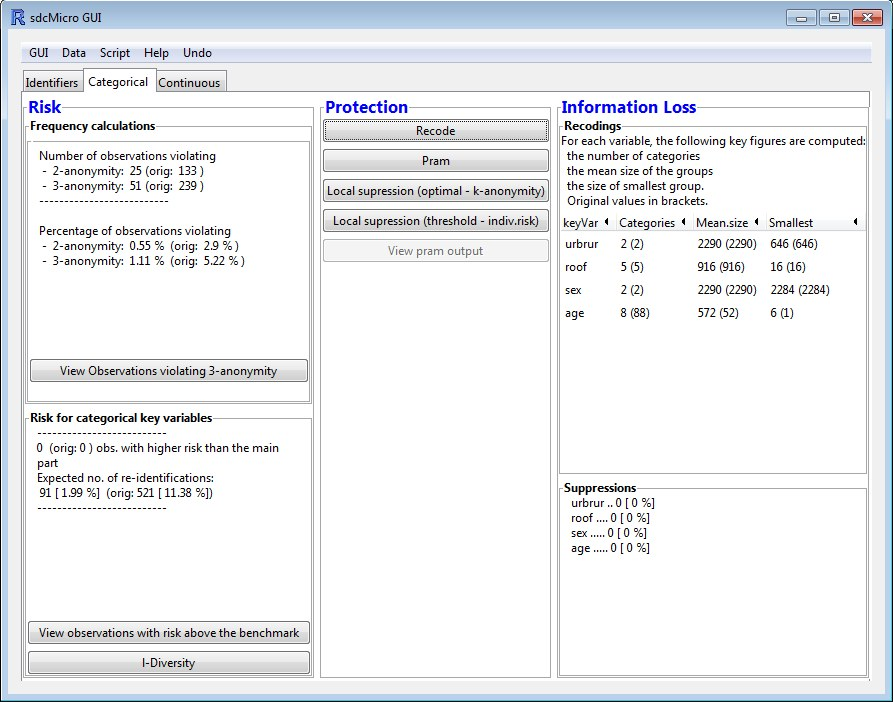
\includegraphics[width=0.7\linewidth]{figures/sdcMicroScreenshot.jpg}
\caption[\texttt{sdcMicro} Graphical User Interface.]{\texttt{sdcMicro} package graphical user interface.}
\label{fig:sdcMicro-gui}
\end{figure}

Some software suites have been developed to provide the SDC tools needed to effectively anonymize the released datasets. The most prominent of these is the \texttt{sdcMicro} package. It is a free R-based open source suite for the generation of protected data for researchers and public use. It can be used for the generation of anonymized data, i.e. for the creation of public and scientific-use files. In addition, various risk estimation methods are included. Moreover, the \texttt{sdcMicro} package it is bundled with a graphical user interface for some of the SDC methods it offers.

The \texttt{sdcMicro} includes all the methods of another popular software, called $\mu$-ARGUS\footnote{The $\mu$-ARGUS suite can be found on \url{http://neon.vb.cbs.nl/casc/mu.htm}, but it seems to be quite an outdated software.}, along with some more new methods. A series of documents can be found on the official website of the package concerning its usage.